% Estrategias propuestas: no son resultados de simulación.
\clearpage
\subsection{Escenario pasivo (C1)}
\label{sec:c1-propuesta}

El escenario C1 se plantea como un paquete organizado en cinco criterios: protección solar exterior, área libre de ventanas, recorrido del aire por el atrio, control de la ventilación natural y aprovechamiento de luz natural. Se ha preparado una copia independiente del modelo base; las medidas descritas a continuación todavía no se han aplicado ni simulado. Por tanto, este apartado define la propuesta de ensayo y no demuestra ahorros energéticos.

Para aislar el efecto de C1, se conservarán la orientación, la materialidad, el clima, la ocupación, las cargas y las consignas del caso base. Los cambios en capas o propiedades térmicas de la envolvente se reservan para C2. La cubierta del atrio y las rejillas superiores forman parte de la configuración base y se mantienen.

\subsubsection{Criterio 1: protección solar exterior}
La primera estrategia consiste en complementar las protecciones donde su cobertura resulte insuficiente. El modelo ya contiene celosías y voladizos, por lo que se debe comprobar su geometría antes de añadir aleros o lamas. La figura~\ref{fig:c1-solar} expresa el criterio de intervención; sus dimensiones se definirán por ventana y orientación. La evaluación conjunta de energía e iluminación permitirá reconocer posibles penalizaciones de luz natural.

\begin{figure}[H]
\centering
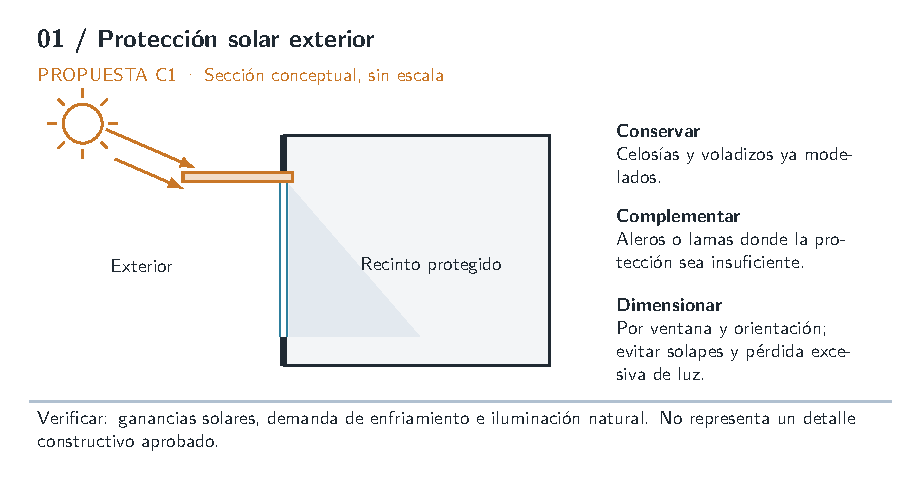
\includegraphics[width=\textwidth]{figuras/c1/c1-proteccion-solar.pdf}
\caption{Criterio propuesto de protección solar exterior para C1.}
\label{fig:c1-solar}
\fuente{Elaboración propia a partir de la revisión del modelo base en DesignBuilder. Esquema conceptual sin escala; geometría adicional pendiente de dimensionamiento.}
\end{figure}

\clearpage
\subsubsection{Criterio 2: área libre de ventanas}
Se propone evaluar una fracción practicable del 20\,\% en ventanas exteriores de oficinas. El valor del 5\,\% se observó en el nivel general del edificio y en la zona 1PA-OF-02; no se extiende automáticamente a todas las ventanas. El 20\,\% constituye un parámetro propuesto de ensayo, pendiente de comprobar mediante el tipo de hoja, el área libre efectiva y su compatibilidad con las celosías.

La figura~\ref{fig:c1-aperturas} distingue el valor observado del parámetro propuesto. La selección de ventanas deberá considerar su operación real, accesibilidad y compatibilidad con las protecciones exteriores.

\begin{figure}[H]
\centering
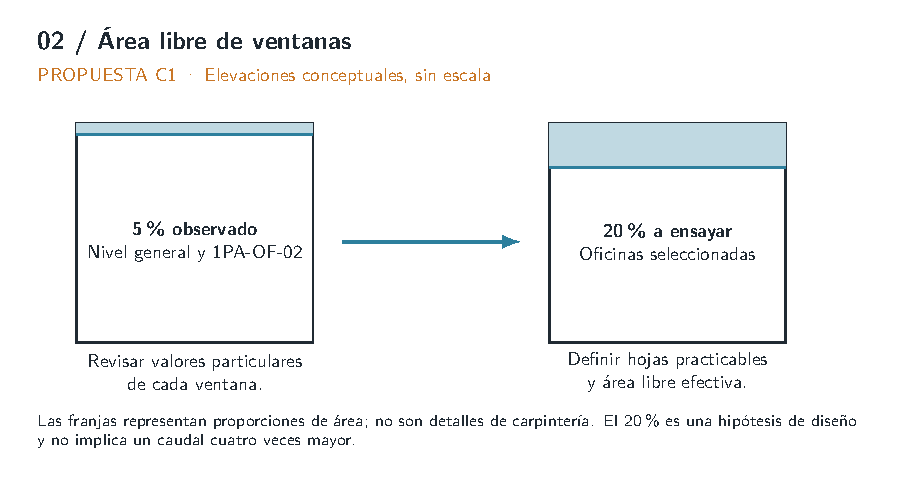
\includegraphics[width=\textwidth]{figuras/c1/c1-aperturas.pdf}
\caption{Fracción de apertura observada y propuesta de ensayo en ventanas de oficinas.}
\label{fig:c1-aperturas}
\fuente{Elaboración propia. Proporciones conceptuales; no representan dimensiones de hojas ni resultados de ventilación.}
\end{figure}

\clearpage
\subsubsection{Criterio 3: recorrido del aire por el atrio}
La figura~\ref{fig:c1-aire} representa el recorrido que se debe verificar entre exterior, oficinas, pasillos y atrio. El atrio comienza en la primera planta alta y conserva su cubierta. Las flechas no representan resultados de caudal ni prueban ventilación cruzada: se comprobarán las conexiones interiores efectivas y la respuesta de la red de flujo de aire. No se presuponen nuevos pasos en divisiones cerradas.

\begin{figure}[H]
\centering
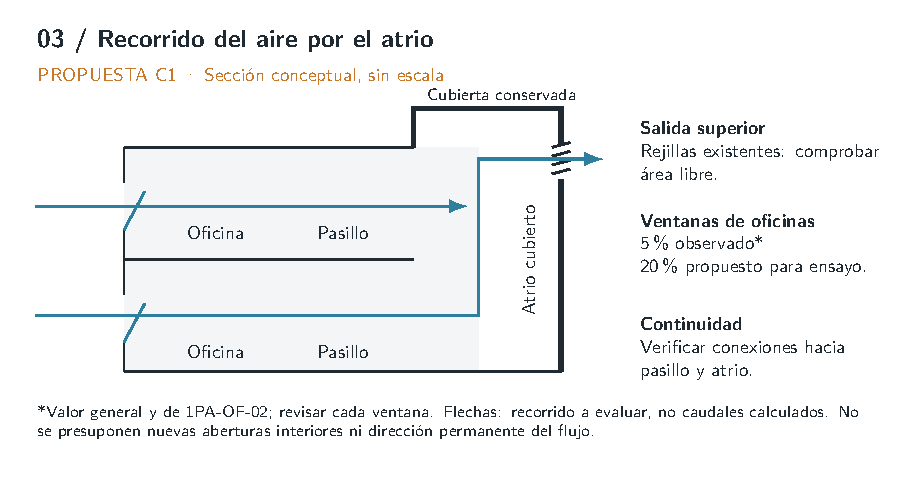
\includegraphics[width=\textwidth]{figuras/c1/c1-ventilacion-atrio.pdf}
\caption{Esquema del recorrido de aire a evaluar y propuesta de apertura de ventanas para C1.}
\label{fig:c1-aire}
\fuente{Elaboración propia. Sección conceptual, sin escala, basada en el atrio cubierto del modelo. Las conexiones, áreas libres y caudales requieren verificación.}
\end{figure}

\clearpage
\subsubsection{Criterio 4: control de la ventilación natural}
El cuarto criterio plantea coordinar la apertura de ventanas con el horario de uso y la demanda de refrigeración. La secuencia de la figura~\ref{fig:c1-control} requiere definir y comprobar los umbrales interiores y exteriores, las restricciones de operación y el comportamiento del sistema cuando se habilita la ventilación natural. Se mantendrán las consignas del caso base para distinguir el efecto de la estrategia.

\begin{figure}[H]
\centering
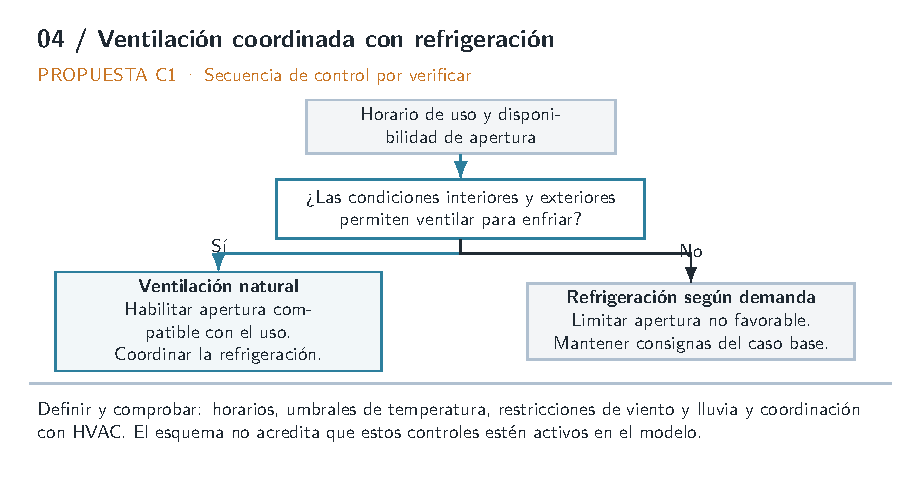
\includegraphics[width=\textwidth]{figuras/c1/c1-control-ventilacion.pdf}
\caption{Secuencia propuesta de coordinación entre ventilación natural y refrigeración para C1.}
\label{fig:c1-control}
\fuente{Elaboración propia. Lógica conceptual pendiente de configuración y verificación en el archivo de simulación; no representa controles ya implementados.}
\end{figure}

La evaluación considerará demanda térmica sensible y total, electricidad estimada de refrigeración, temperaturas durante horas ocupadas y ventilación por zona. La iluminación natural se recalculará con las mismas condiciones del caso base. Los resultados heredados al copiar el archivo no se utilizarán como resultados de C1.

\clearpage
\subsubsection{Criterio 5: aprovechamiento de luz natural}
El quinto criterio consiste en ajustar la geometría de las protecciones para equilibrar el control solar y la entrada de luz natural, como se representa en la figura~\ref{fig:c1-luz}. Se evaluarán profundidad y separación de aleros o lamas, manteniendo el vidrio y las reflectancias del caso base. Este criterio complementa la protección solar y no constituye una sustitución de materiales.

La comparación se realizará con cielo CIE cubierto de 10000 lux, plano de trabajo a 0,76 m y malla de 0,30 m. Se revisarán la distribución de iluminancia y la proporción de área que supera FLD 2\,\%. Este ensayo estático no permite afirmar autonomía lumínica anual ni ausencia de deslumbramiento. Tampoco se atribuirá ahorro de electricidad de iluminación sin modelar y evaluar el control correspondiente.

\begin{figure}[H]
\centering
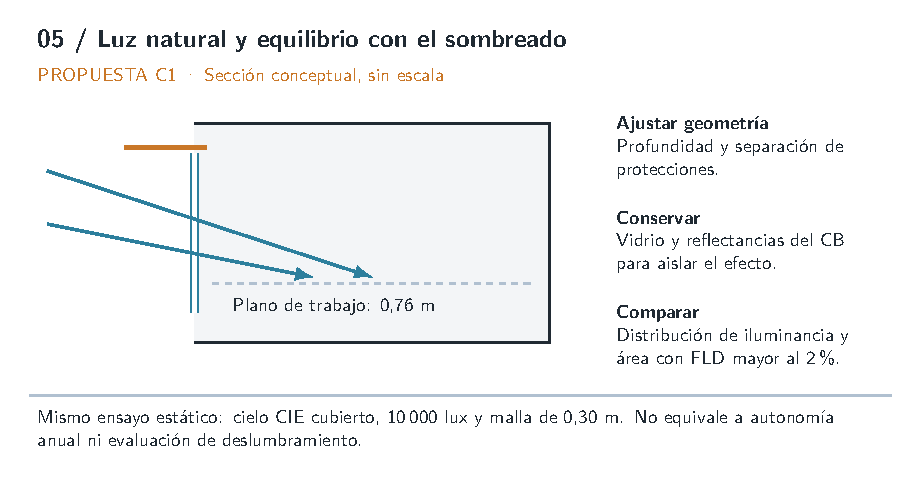
\includegraphics[width=\textwidth]{figuras/c1/c1-iluminacion-natural.pdf}
\caption{Criterio de equilibrio entre protección solar y aprovechamiento de luz natural.}
\label{fig:c1-luz}
\fuente{Elaboración propia. Sección conceptual; condiciones de cálculo equivalentes al ensayo estático del caso base.}
\end{figure}

Los cinco criterios se evaluarán como un paquete C1. El área libre, el recorrido del aire y su control son aspectos complementarios de la ventilación; una sola corrida conjunta no permite atribuir por separado los ahorros a cada criterio. Para ello serían necesarios ensayos adicionales modificando una variable cada vez.

\clearpage
\subsubsection{Registro de intervención y validación}
La tabla~\ref{tab:c1-paquete} distingue las condiciones observadas de las decisiones propuestas. Antes de la comparación final se deberán resolver o justificar las incidencias del caso base relativas al datacenter, al dimensionamiento de invierno y a la geometría de la red de aire. Cualquier corrección de una entrada común exigirá actualizar también la simulación base.

\begin{table}[H]
\centering
\caption{Parámetros y verificaciones del paquete pasivo C1.}
\label{tab:c1-paquete}
{\fontsize{9}{11}\selectfont
\begin{tabular}{p{2.4cm}p{3.1cm}p{3.1cm}p{3.1cm}}
\toprule
Medida & Condición base & Propuesta C1 & Verificación pendiente \\
\midrule
Protección solar & Celosías y voladizos modelados. & Complementar protección insuficiente. & Dimensiones, orientación, solapes y luz natural. \\
\addlinespace
Ventanas & Apertura de 5\,\% observada a nivel general y en 1PA-OF-02. & Ensayar 20\,\% en ventanas de oficinas seleccionadas. & Inventario por ventana, tipo de hoja y área libre. \\
\addlinespace
Atrio & Cubierta, pasos abiertos y rejillas superiores. & Conservar y verificar el recorrido del aire. & Conectividad, aberturas horizontales y caudales. \\
\addlinespace
Operación & Controles particulares del modelo base. & Coordinar ventanas y refrigeración. & Horarios, umbrales y control exportado. \\
\addlinespace
Luz natural & Ensayo estático actualizado del CB. & Ajustar protecciones conservando vidrio y reflectancias. & Iluminancia y área con FLD mayor al 2\,\%. \\
\bottomrule
\end{tabular}}
\fuente{Elaboración propia a partir de la revisión del modelo y de la propuesta de ensayo. Ninguna fila acredita una medida simulada.}
\end{table}

La validación seguirá la secuencia: definir el paquete, aplicar los cambios en la copia C1, contrastar el archivo exportado con CB, ejecutar las simulaciones y comparar los indicadores. La combinación de medidas pasivas con sustituciones de materiales corresponderá a C3, después de evaluar C1 y C2 por separado.

\clearpage
